%% bare_conf.tex
%% V1.4b
%% 2015/08/26
%% by Michael Shell
%% See:
%% http://www.michaelshell.org/
%% for current contact information.
%%
%% This is a skeleton file demonstrating the use of IEEEtran.cls
%% (requires IEEEtran.cls version 1.8b or later) with an IEEE
%% conference paper.
%%
%% Support sites:
%% http://www.michaelshell.org/tex/ieeetran/
%% http://www.ctan.org/pkg/ieeetran
%% and
%% http://www.ieee.org/

%%*************************************************************************
%% Legal Notice:
%% This code is offered as-is without any warranty either expressed or
%% implied; without even the implied warranty of MERCHANTABILITY or
%% FITNESS FOR A PARTICULAR PURPOSE! 
%% User assumes all risk.
%% In no event shall the IEEE or any contributor to this code be liable for
%% any damages or losses, including, but not limited to, incidental,
%% consequential, or any other damages, resulting from the use or misuse
%% of any information contained here.
%%
%% All comments are the opinions of their respective authors and are not
%% necessarily endorsed by the IEEE.
%%
%% This work is distributed under the LaTeX Project Public License (LPPL)
%% ( http://www.latex-project.org/ ) version 1.3, and may be freely used,
%% distributed and modified. A copy of the LPPL, version 1.3, is included
%% in the base LaTeX documentation of all distributions of LaTeX released
%% 2003/12/01 or later.
%% Retain all contribution notices and credits.
%% ** Modified files should be clearly indicated as such, including  **
%% ** renaming them and changing author support contact information. **
%%*************************************************************************


% *** Authors should verify (and, if needed, correct) their LaTeX system  ***
% *** with the testflow diagnostic prior to trusting their LaTeX framework ***
% *** with production work. The IEEE's font choices and paper sizes can   ***
% *** trigger bugs that do not appear when using other class files.       ***                          ***
% The testflow support page is at:
% http://www.michaelshell.org/tex/testflow/


\label{beginning of document}
\documentclass[10pt,conference]{IEEEtran}
% Some Computer Society conferences also require the compsoc mode option,
% but others use the standard conference format.
%
% If IEEEtran.cls has not been installed into the LaTeX system files,
% manually specify the path to it like:
% \documentclass[conference]{../sty/IEEEtran}

\usepackage{graphicx}
	\graphicspath{{images/}} 
\renewcommand\IEEEkeywordsname{Keywords}
\usepackage{hyperref}
	\hypersetup{colorlinks=true,allcolors=blue}
\usepackage{hypcap}
\usepackage{caption}
\usepackage{subcaption}
\usepackage{listings}
\lstset{
 		basicstyle=\ttfamily\scriptsize,
 		%frame=single,
 		breaklines=true,
 		numbers=left,
 		xleftmargin=2.5em,
 		framexleftmargin=0em,
 		emph={
       	class, extends, operation, abstract,
       	context, constraint, check,
       	for, if, return, true, and, ref,
       	message, in, package, val, attr, 
       	@link, @node, @compartment,
       	@namespace, @diagram
   	},
   	emphstyle=\textbf
}
\lstdefinestyle{interfaces}{
 		float=t
}
\lstdefinestyle{java}{
    basicstyle=\ttfamily\scriptsize,
    emph={
        case, $unset$,
        instanceof, else, if, void,
        new, UnsetEAttributeEvent,
        UnsetEReferenceEvent,
        @override, public, class, extends
    }
}

% correct bad hyphenation here
\hyphenation{op-tical net-works semi-conduc-tor}


\begin{document}
%
% paper title
% Titles are generally capitalized except for words such as a, an, and, as,
% at, but, by, for, in, nor, of, on, or, the, to and up, which are usually
% not capitalized unless they are the first or last word of the title.
% Linebreaks \\ can be used within to get better formatting as desired.
% Do not put math or special symbols in the title.
\title{Hybrid Model Persistence}


% author names and affiliations
% use a multiple column layout for up to three different
% affiliations\ref{abstract}
\author{\IEEEauthorblockN{Alfa Yohannis\IEEEauthorrefmark{1}, Horacio Hoyos Rodriguez\IEEEauthorrefmark{2}, Fiona Polack\IEEEauthorrefmark{3}, Dimitris Kolovos\IEEEauthorrefmark{4}}
\IEEEauthorblockA{
    \IEEEauthorrefmark{1}\IEEEauthorrefmark{2}\IEEEauthorrefmark{4}Department of Computer Science, University of York, York, United Kingdom \\
    \IEEEauthorrefmark{3}School of Computing and Maths, Keele University, United Kingdom \\
Email: \IEEEauthorrefmark{1}ary506@york.ac.uk, \IEEEauthorrefmark{2}horacio\_hoyos\_rodriguez@ieee.org, \\
\IEEEauthorrefmark{3}f.a.c.polack@keele.ac.uk, \IEEEauthorrefmark{4}dimitris.kolovos@york.ac.uk}}

% conference papers do not typically use \thanks and this command
% is locked out in conference mode. If really needed, such as for
% the acknowledgment of grants, issue a \IEEEoverridecommandlockouts
% after \documentclass

% for over three affiliations, or if they all won't fit within the width
% of the page, use this alternative format:
% 
%\author{\IEEEauthorblockN{Michael Shell\IEEEauthorrefmark{1},
%Homer Simpson\IEEEauthorrefmark{2},
%James Kirk\IEEEauthorrefmark{3}, 
%Montgomery Scott\IEEEauthorrefmark{3} and
%Eldon Tyrell\IEEEauthorrefmark{4}}
%\IEEEauthorblockA{\IEEEauthorrefmark{1}School of Electrical and Computer Engineering\\
%Georgia Institute of Technology,
%Atlanta, Georgia 30332--0250\\ Email: see http://www.michaelshell.org/contact.html}
%\IEEEauthorblockA{\IEEEauthorrefmark{2}Twentieth Century Fox, Springfield, USA\\
%Email: homer@thesimpsons.com}
%\IEEEauthorblockA{\IEEEauthorrefmark{3}Starfleet Academy, San Francisco, California 96678-2391\\
%Telephone: (800) 555--1212, Fax: (888) 555--1212}
%\IEEEauthorblockA{\IEEEauthorrefmark{4}Tyrell Inc., 123 Replicant Street, Los Angeles, California 90210--4321}}




% use for special paper notices
%\IEEEspecialpapernotice{(Invited Paper)}




% make the title area
\maketitle

% As a general rule, do not put math, special symbols or citations
% in the abstract
\begin{abstract}
\label{abstract}
Lorem ipsum dolor sit amet consectetur adipiscing elit malesuada sollicitudin, penatibus ultricies primis accumsan volutpat id aliquet orci, netus congue tempus ligula proin ornare laoreet pharetra. Fringilla nibh felis odio duis tincidunt eget ultricies tellus, eros molestie phasellus lacinia accumsan mus gravida conubia, purus at posuere tristique porttitor volutpat sociis. Varius duis facilisi condimentum rhoncus nascetur velit cum nostra, cubilia ridiculus a himenaeos massa sem inceptos, dignissim in nibh elementum interdum nisi ligula.
\end{abstract}
%
% no keywords
\begin{IEEEkeywords} 
model persistence, hybrid persistence, change-based persistence, state-based persistence
\end{IEEEkeywords}

% For peer review papers, you can put extra information on the cover
% page as needed:
% \ifCLASSOPTIONpeerreview
% \begin{center} \bfseries EDICS Category: 3-BBND \end{center}
% \fi
%
% For peerreview papers, this IEEEtran command inserts a page break and
% creates the second title. It will be ignored for other modes.
\IEEEpeerreviewmaketitle

\section{Introduction}
\label{sec:introduction}
Change-based model persistence \cite{DBLP:conf/models/YohannisKP17} comes with at least two main advantages: it provides support for (1) fast comparison of versions of the same model \cite{DBLP:conf/sde/LippeO92,DBLP:conf/caise/IgnatN05,DBLP:conf/edoc/KoegelHLHD10,koegel2010emfstore}  -- which can also substantially speed up incremental model management activities, and (2) recording fine-grained changes in models that can enable model analytics (e.g. understand how modellers use modelling languages and tools) \cite{DBLP:journals/entcs/RobbesL07}. However, the approach comes with cost: the ever-growing model files \cite{DBLP:conf/edoc/KoegelHLHD10,DBLP:journals/entcs/RobbesL07} and increased loading time \cite{mens2002state}. In this work we are addressing the former by introducing the concept of hybrid model persistence. In hybrid model persistence the change-based representation is augmented with a state-based representation of the latest snapshot of the model which is used to speed up model loading and querying. We investigate the impact of the hybrid model persistence on model loading and saving time, memory footprint on loading and saving a model, and storage space usage, and argue that hybrid model persistence is a fair trade-off for state-based persistence.
 
The rest of the paper is structured as follows. Section \ref{sec:change_based_model_persistence} introduces a running example and provides a brief introduction to change-based model persistence.
Section \ref{sec:hybrid_model_persistence} presents our approach to hybrid model persistence. Section \ref{sec:evaluation} presents experimental results and evaluation. Section \ref{sec:related_work} provides an overview of related work, and Section \ref{sec:conlcusions_and_future_work} concludes with a discussion on directions of future work.


\section{Change-based Model Persistence}
\label{sec:change_based_model_persistence}

\section{Hybrid Model Persistence}
\label{sec:hybrid_model_persistence}
Hybrid model persistence is essentially combining two types of persistence, change-based and state-based model persistence, to work together side-by-side. When a model is modified, the occurred changes are recorded into both representations of persistence. The former persists all the changes to keep the model's history, while the latter is used to maintain the last state of the model produced by the changes. In terms of loading, the model is directly loaded from the state-based representation. Thus, replaying all the changes from its change-based representation -- which is time consuming -- to get the last state of the model can be avoided.

These ideas are then translated into an inplementation that conforms to metamodelling architectures such as MOF \cite{omg2018mof} and EMF \cite{steinberg2008emf}. The work is derived from an existing implementation of change-based model persistence, the Epsilon CBP \cite{DBLP:conf/models/YohannisKP17}, and augmented with two state-based persistence implementations, NeoEMF \cite{daniel2016neoemf} and XMI \cite{omg2018xmi}. The design of our implementation follows the class diagram presented in Fig. \ref{fig:class_diagram}. 

\begin{figure}[ht]
    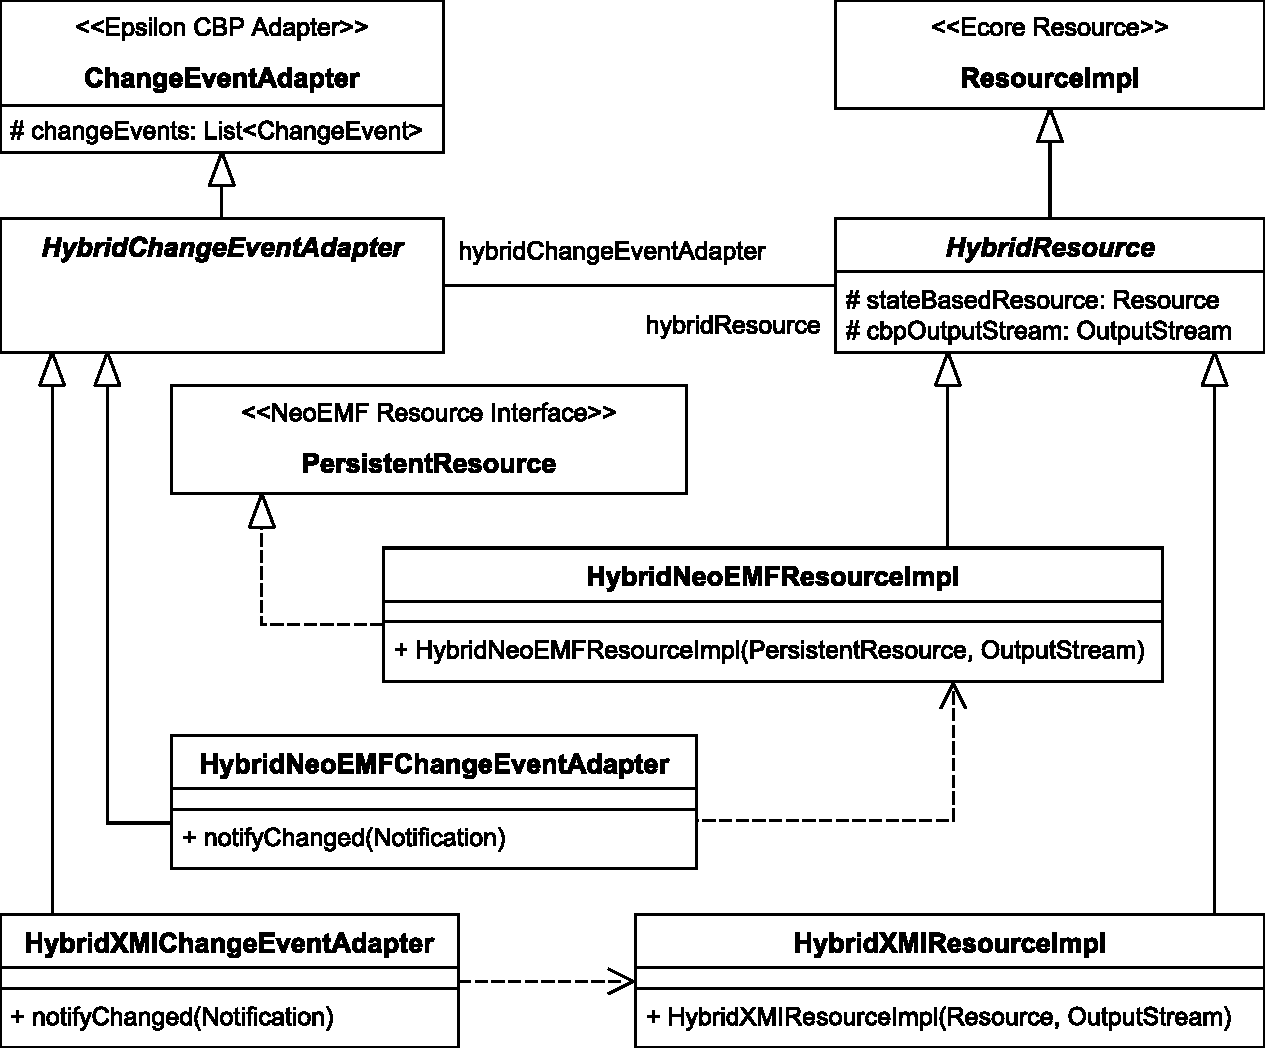
\includegraphics[width=\linewidth]{images/class_diagram}
    \caption{The class diagram of hybrid model persistence.}
    \label{fig:class_diagram}
\end{figure}

The Epsilon CBP provides a $ChangeEventAdapter$ class, an derived $EContentAdapter$ adapter class that collects changes made to a model in the form a list of events, $changeEvents$. The events occur when the model is modified and are recorded by the class. Based on this class, we derives another adapter class, $ChangeHybridEventAdapter$, for the hybrid model persistence. It is an abstract class so that it can be further derived to create different implementations of adapter classes for different types of state-based persistence. The $ChangeHybridNeoEMFEventAdapater$ is the adapter class for NeoEMF and the $ChangeHybridXMIEventAdapater$ for XMI. These classes override the $notifyChanged(Notification)$ that belongs to the $ChangeEventAdapter$ class to handle events that are specific to NeoEMF and XMI respectively. 

We also create a resource class for hybrid persistence, the $HybridResource$ class. The class is made abstract so that it can be realised in different resource implementation classes for different state-based persistence (e.g. NeoEMF and XMI). The $HybridResource$ class contains the $stateBasedResource$ attribute which is used to refer to a state-based persistence that is being used, and the $cbpOutputStream$ attribute that refers to an $OutputStream$ (e.g. file, in-memory) as the representation of the change-based persistence for saving changes. This $HybridResource$ class has an association with the $HybridChangeEventAdapater$ class so that the former class can access the events collected by the latter class, and the latter class can also use functionalities provided by the former class (e.g. getting the id of an element in the resource, saving changes to a change-based model representation).

The resource implementation class for NeoEMF is the $HybridNeoEMFResourceImpl$ class, and $HybridXMIResourceImpl$ class for XMI. Both are derived from the $HybridPersistence$. Their constructors take two parameters: a $PersistentResource$ for NeoEMF or $Resource$ for XMI, and an $OutputStream$ of a change-based model persistence. These two inputs are assigned to the derived $stateBasedResource$ and $cbpOutputStream$ attributes respectively. For $HybridNeoEMFResourceImpl$ , this class also implements the NeoEMF's $HybridPersistence$ interface so that specific NeoEMF's methods can also be implemented on this hybrid implementation class (e.g. $close$() method to close a connection with a backend database). 

Inside the $HybridNeoEMFResourceImpl$'s constructor, a $HybridChangeEventAdapater$ is registered to the NeoEMF resource's $eAdapters$ in order for the adapter can listen to changes (Fig. \ref{lst:attach_adapater_neo}). The same procedure is also applied to XMI in order for the adapter to work (Fig. \ref{lst:attach_adapater_xmi}). 

\begin{lstlisting}[style=java,caption={A simplified code to connect a change-based model persistence's event adapater to a NeoEMF resource.},label=lst:attach_adapater_neo]
public HybridNeoEMFResourceImpl(PersistentResource persistentResource, OutputStream outputStream) throws IOException {
    ...
    this.stateBasedResource = persistentResource;
    hybridChangeEventAdapter = new HybridNeoEMFChangeEventAdapter(this);
    stateBasedResource.eAdapters().add(hybridChangeEventAdapter);
    ...
}
\end{lstlisting}

\begin{lstlisting}[style=java,caption={A simplified code to connect a change-based model persistence's event adapater to an XMI resource.},label=lst:attach_adapater_xmi]
public HybridXMIResourceImpl(Resource resource, OutputStream outputStream) throws IOException {
...
this.stateBasedResource = resource;
hybridChangeEventAdapter = new HybridXMIChangeEventAdapter(this);
stateBasedResource.eAdapters().add(hybridChangeEventAdapter);
...
}
\end{lstlisting}

Basically, the hybrid model persistence only executes the code in List. \ref{lst:hybrid_load_neo} to load a model. It overrides the $load$ method of the $ResourceImpl$ class (line 1-2) and executes the load method of the NeoEMF resource (line 4). The same steps also apply to hybrid model persistence with XMI resource, except that it overrides the $doLoad$ method of the $ResourceImpl$, in order to load properly (List. \ref{lst:hybrid_load_xmi}). 

\begin{lstlisting}[style=java,caption={The simplified $load$ method of the hybrid model persistence with NeoEMF as its state-based resource.},label=lst:hybrid_load_neo]
@Override
public void load(Map<?, ?> options) throws IOException {
    ... 
    stateBasedResource.load(options);
    ...
}
\end{lstlisting}

\begin{lstlisting}[style=java,caption={The simplified $load$ method of the hybrid model persistence with XMI as its state-based resource.},label=lst:hybrid_load_xmi]
@Override
public void doLoad(Map<?, ?> options) throws IOException {
    ... 
    stateBasedResource.load(options);
    ...
}
\end{lstlisting}

In saving a model, the  $HybridNeoEMFResourceImpl$ and $HybridXMIResourceImpl$ overrides the $save$ and $doSave$ method of the $ResourceImpl$ class (List. \ref{lst:hybrid_save_neo} and \ref{lst:hybrid_save_xmi}, line 1-2). Inside both methods, both resources execute the $save$ method of their state-based persistence (line 4) and execute the $saveChangeBasedPersitence$ method to save changes made to a model to a change-based representation represented by the $cbpOutputStream$.

\begin{lstlisting}[style=java,caption={A simplified code to save a model to both state and change-based representation of the hybrid model persistence.},label=lst:hybrid_save_neo]
@Override
public void save(Map<?, ?> options) throws IOException {
    ...
    stateBasedResource.save(options);
    saveChangeBasedPersistence(cbpOutputStream, options);
    ...
}
\end{lstlisting}

\begin{lstlisting}[style=java,caption={A simplified code to save a model to both state and change-based representation of the hybrid model persistence.},label=lst:hybrid_save_xmi]
@Override
public void doSave(Map<?, ?> options) throws IOException {
    ...
    stateBasedResource.save(options);
    saveChangeBasedPersistence(cbpOutputStream, options);
    ...
}
\end{lstlisting}

\section{Evaluation}
\label{sec:evaluation}

In this section, we compare hybrid model persistence (Epsilon CBP and NeoEMF or XMI) vs. state-based persistence (NeoEMF or XMI only) on loading, saving, and storage space usage of models and argue that hybrid model persistence offers a fair trade-off for the latter. 

\subsection{Evaluation Method}
\label{sec:evaluation_method}
We developed the prototype of the proposed hybrid model persistence approach\footnote{The prototype, tests, and data used in the evaluation are available under \url{https://github.com/epsilonlabs/emf-cbp} and \url{https://goo.gl/1zUBQC}.}. The evaluation was performed on Intel\textsuperscript{\textregistered} Core\textsuperscript{TM} i7-6500U CPU@2.50GHz 2.59GHz, 12GB RAM, and the Java\textsuperscript{TM} SE Runtime Environment (build 1.8.0\textunderscore162-b12).

For the evaluation, we used synthetic hybrid models derived from a real-world project, the Epsilon \cite{eclipse2017epsilon,eclipse2018epsilongit}. For state-based representation of the models, we used MoDisco \cite{DBLP:journals/infsof/BruneliereCDM14} to generate XMI-based UML2 \cite{eclipse2017uml2} models that reflect the source code of the project and then imported the generated models into NeoEMF. While obtaining the state-based part is trivial, obtaining its change-based part that reflects the changes of a real-world project was not straightforward. The change-based part was derived from the diffs identified from the subsequent versions of the project committed on its Git repository. Since the project have many committed versions, different models can be generated, and to some degree, they reflect the time-ordered changes of the cases. The change-based representation was derived by comparing an initially-empty running model to the generated models sequentially, version-by-version. All identified differences were then reconciled by performing a unidirectional merging to the running model. All changes made to the running model during the merging process were captured and persisted into a CBP file. EMF Compare was used \cite{eclipse2017compare} to perform the comparison and merging.

Using the models, we performed performance evaluation on loading time, saving time, and memory footprint for both loading and saving. We compared the performance of the hybrid approach against state-based-only approach. For loading and saving time, we measured the delta time required to complete the loading and saving. For memory footprint, we measured the delta of memory used before and after loading and saving completes. Specifically for saving, we measured the time and memory footprint required to save a new version of a model, after one single change has been made to the model. We also measured the impact of using the hybrid approach on the execution time of a model comparison, specifically for identifying differences between a model and its preceding versions. The hybrid approach was compared to model-to-model comparison using EMF Compare on their execution time.

We performed measurement 22 times for each dimension measured. The results of the measurement enabled us to perform the Welch's t-test \cite{welch1947ttest} to find the significance of the comparisons for each case. We used a significance level of 5\%. If t-test' $p$-$value$ $<$ 0.05, we rejected the null hypothesis -- the $means$ of the compared persistence types are equal ($H_0$) -- and accepted the alternative hypothesis -- the $means$ of the compared persistence types are not equal ($H_1$).  

\subsection{Loading Time and Memory Footprint}
\label{sec:model_loading_time}


\begin{figure}[ht]
        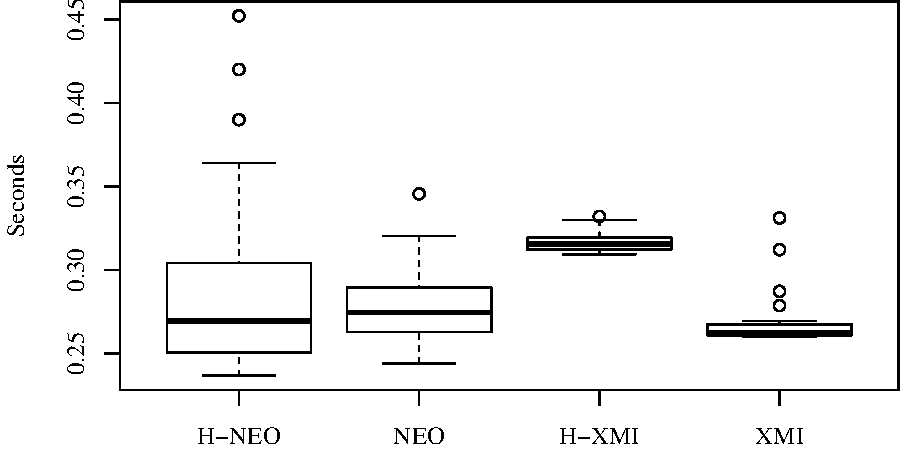
\includegraphics[width=\linewidth]{images/load_time_epsilon}
    \caption{Hybrid vs. state-based model persistence on model loading time.}
            \label{fig:load_time_epsilon}
\end{figure}

\begin{figure}[ht]
        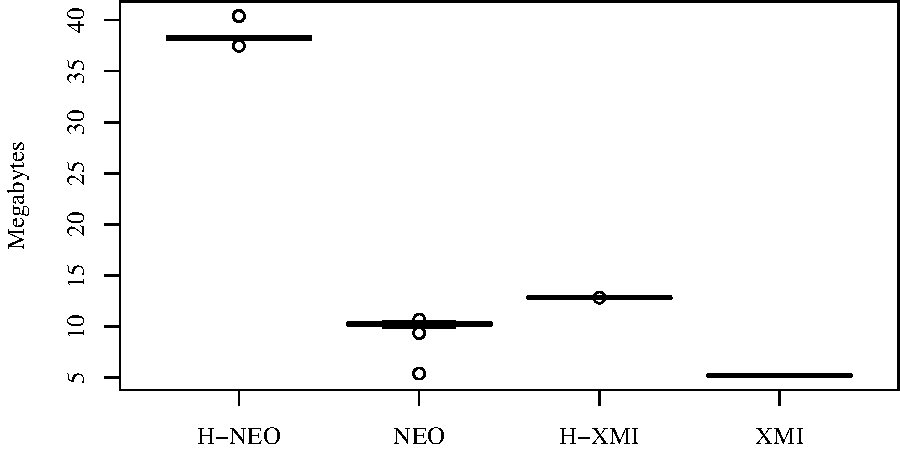
\includegraphics[width=\linewidth]{images/load_memory_epsilon}
        \caption{loading memory footprint}
    \caption{Hybrid vs. state-based model persistence on the memory footprint of loading a model.}
\label{fig:load_memory_epsilon}
\end{figure}


\subsection{Model Saving Time and Memory Footprint}
\label{sec:model_saving_time}

\begin{figure}[ht]
    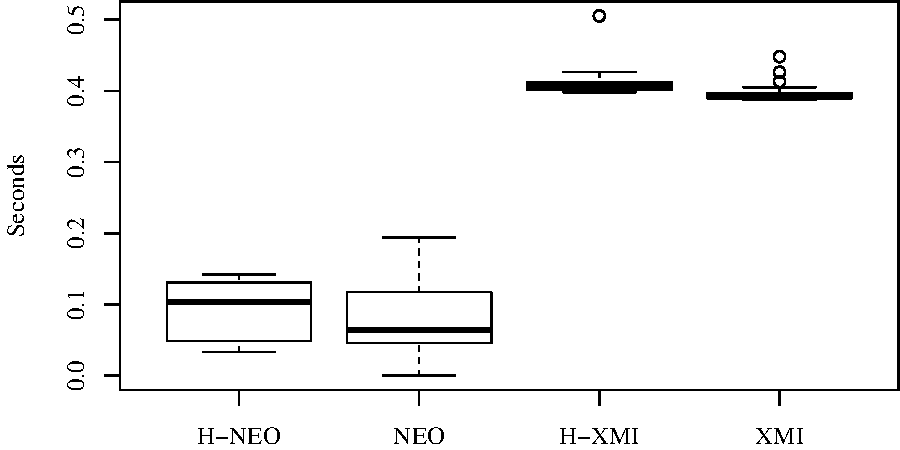
\includegraphics[width=\linewidth]{images/save_time_epsilon}
    \caption{Hybrid vs. state-based model persistence on model saving time.}
    \label{fig:save_time_epsilon}
\end{figure}
\ref{fig:save_memory_epsilon}
\begin{figure}[ht]
    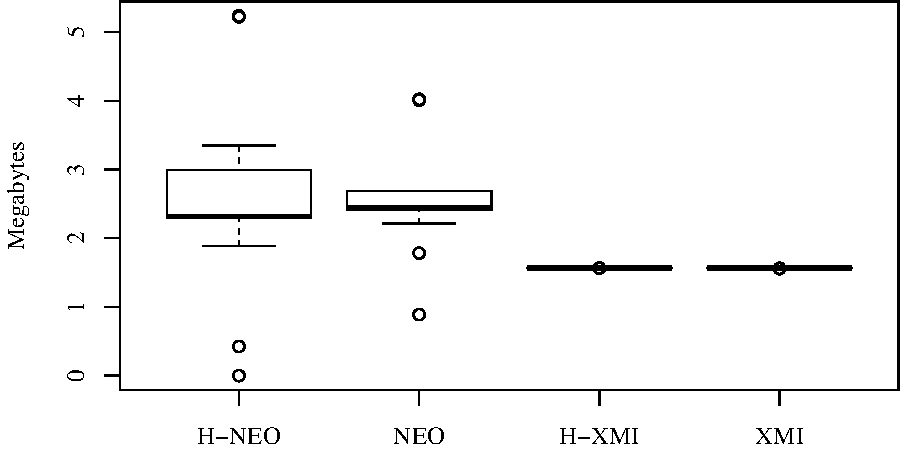
\includegraphics[width=\linewidth]{images/save_memory_epsilon}
    \caption{Hybrid vs. state-based model persistence on the memory footprint of saving a model.}
    \label{fig:save_memory_epsilon}
\end{figure}


\subsection{Storage Space Usage}
\label{sec:storage_space_usage}

\begin{table} [ht]
    \centering
    \caption{Space Usage for the BPMN2 project. The CBP were generated from version 1 to 192 of the project.}
    \label{table:space_usage_bpmn2}
    \begin{tabular}{ p{0.1\linewidth} p{0.1\linewidth} p{0.12\linewidth} p{0.13\linewidth} p{0.26\linewidth} }
        \hline 
        \textbf{Type} & \textbf{Element Count} & \textbf{Event Count} & \textbf{Size} & \textbf{Average} \\
        \hline 
        XMI & 62,062 &  & 6.55 MBs & 110 bytes / element  \\
        NeoEMF & 62,062 &  & 134 MBs & 2 KBs / element \\
        CBP &  & 1,238,751 & 109 MBs &  92 bytes / event \\
        \hline 
    \end{tabular}
\end{table}

\begin{table} [ht]
    \centering
    \caption{Space Usage for the Epsilon project. The CBP were generated from  version 1 to 940 of the project.}
    \label{table:space_usage_epsilon}
    \begin{tabular}{ p{0.1\linewidth} p{0.1\linewidth} p{0.12\linewidth} p{0.13\linewidth} p{0.26\linewidth} }
    \hline 
    \textbf{Type} & \textbf{Element Count} & \textbf{Event Count} & \textbf{Size} & \textbf{Average} \\
    \hline 
    XMI & 88,020 &  & 9.44 MBs & 112 bytes / element  \\
    NeoEMF & 88,020 &  & 188 MBs & 2 KBs / element \\
    CBP &  & 4,307,051 & 406 MBs &  98 bytes / event \\
    \hline 
    \end{tabular}
\end{table}

\begin{table} [ht]
    \centering
    \caption{Space Usage for the Wikipedia's US article. The CBP were generated from version 1 to 10187 of the article.}
    \label{table:space_usage_Wikipedia}
    \begin{tabular}{ p{0.1\linewidth} p{0.1\linewidth} p{0.12\linewidth} p{0.13\linewidth} p{0.26\linewidth} }
        \hline 
        \textbf{Type} & \textbf{Element Count} & \textbf{Event Count} & \textbf{Size} & \textbf{Average} \\
        \hline 
        XMI & 13,112 &  & 1.28 MBs & 102 bytes / element  \\
        NeoEMF & 13,112 &  & 31.8 MBs & 2 KBs / element \\
        CBP &  & 62,271,003 & 5.85 GBs &  98 bytes / event \\
        \hline 
    \end{tabular}
\end{table}

\subsection{Change Detection}
\label{sec:change_detection}



\section{Discussion}
\label{sec:discussion}

\section{Related Work}
\label{sec:related_work}
 There are several non-XMI approaches to state-based model persistence, using relational or NoSQL databases. For example, EMF Teneo\,\cite{eclipse2017teneo} persists EMF models in relational databases, while Morsa \cite{DBLP:conf/models/Espinazo-PaganCM11} and NeoEMF \cite{daniel2016neoemf} persist models in document and graph databases, respectively.  None of these approaches provides built-in support for versioning and models are eventually stored in binary files/folders which are known to be a poor fit for text-oriented version control systems like Git and SVN. Connected Data Objects (CDO) \cite{eclipse2017cdo}, provides support for database-backed model persistence as well as collaboration facilities, but its adoption necessitates the use of a separate version control system in the software development process (e.g. a Git repository for code and a CDO repository for models), which introduces fragmentation and administration challenges \cite{barmpis2014evaluation}. Similar challenges arise in relation to other model-specific version control systems such as EMFStore\,\cite{koegel2010emfstore}.

\section{Conclusions and Future Work}
\label{sec:conlcusions_and_future_work}


% An example of a floating figure using the graphicx package.
% Note that \label must occur AFTER (or within) \caption.
% For figures, \caption should occur after the \includegraphics.
% Note that IEEEtran v1.7 and later has special internal code that
% is designed to preserve the operation of \label within \caption
% even when the captionsoff option is in effect. However, because
% of issues like this, it may be the safest practice to put all your
% \label just after \caption rather than within \caption{}.
%
% Reminder: the "draftcls" or "draftclsnofoot", not "draft", class
% option should be used if it is desired that the figures are to be
% displayed while in draft mode.
%
%\begin{figure}[!t]
%\centering
%\includegraphics[width=2.5in]{myfigure}
% where an .eps filename suffix will be assumed under latex, 
% and a .pdf suffix will be assumed for pdflatex; or what has been declared
% via \DeclareGraphicsExtensions.
%\caption{Simulation results for the network.}
%\label{fig_sim}
%\end{figure}

% Note that the IEEE typically puts floats only at the top, even when this
% results in a large percentage of a column being occupied by floats.


% An example of a double column floating figure using two subfigures.
% (The subfig.sty package must be loaded for this to work.)
% The subfigure \label commands are set within each subfloat command,
% and the \label for the overall figure must come after \caption.
% \hfil is used as a separator to get equal spacing.
% Watch out that the combined width of all the subfigures on a 
% line do not exceed the text width or a line break will occur.
%
%\begin{figure\\}[!t]
%\centering
%\subfloat[Case I]{\includegraphics[width=2.5in]{box}%
%\label{fig_first_case}}
%\hfil
%\subfloat[Case II]{\includegraphics[width=2.5in]{box}%
%\label{fig_second_case}}
%\caption{Simulation results for the network.}
%\label{fig_sim}
%\end{figure\\}
%
% Note that often IEEE papers with subfigures do not employ subfigure
% captions (using the optional argument to \subfloat[]), but instead will
% reference/describe all of them (a), (b), etc., within the main caption.
% Be aware that for subfig.sty to generate the (a), (b), etc., subfigure
% labels, the optional argument to \subfloat must be present. If a
% subcaption is not desired, just leave its contents blank,
% e.g., \subfloat[].


% An example of a floating table. Note that, for IEEE style tables, the
% \caption command should come BEFORE the table and, given that table
% captions serve much like titles, are usually capitalized except for words
% such as a, an, and, as, at, but, by, for, in, nor, of, on, or, the, to
% and up, which are usually not capitalized unless they are the first or
% last word of the caption. Table text will default to \footnotesize as
% the IEEE normally uses this smaller font for tables.
% The \label must come after \caption as always.
%
%\begin{table}[!t]
%% increase table row spacing, adjust to taste
%\renewcommand{\arraystretch}{1.3}
% if using array.sty, it might be a good idea to tweak the value of
% \extrarowheight as needed to properly center the text within the cells
%\caption{An Example of a Table}
%\label{table_example}
%\centering
%% Some packages, such as MDW tools, offer better commands for making tables
%% than the plain LaTeX2e tabular which is used here.
%\begin{tabular}{|c||c|}
%\hline
%One & Two\\
%\hline
%Three & Four\\
%\hline
%\end{tabular}
%\end{table}


% Note that the IEEE does not put floats in the very first column
% - or typically anywhere on the first page for that matter. Also,
% in-text middle ("here") positioning is typically not used, but it
% is allowed and encouraged for Computer Society conferences (but
% not Computer Society journals). Most IEEE journals/conferences use
% top floats exclusively. 
% Note that, LaTeX2e, unlike IEEE journals/conferences, places
% footnotes above bottom floats. This can be corrected via the
% \fnbelowfloat command of the stfloats package.



% conference papers do not normally have an appendix


% use section\\ for acknowledgment
\section*{Acknowledgments}
This research is part of a doctoral programme funded by \emph{Lembaga Pengelola Dana Pendidikan Indonesia} (Indonesia Endowment Fund for Education).

% trigger a \newpage just before the given reference
% number - used to balance the columns on the last page
% adjust value as needed - may need to be readjusted if
% the document is modified later
%\IEEEtriggeratref{8}
% The "triggered" command can be changed if desired:
%\IEEEtriggercmd{\enlargethispage{-5in}}

% references section

% can use a bibliography generated by BibTeX as a .bbl file
% BibTeX documentation can be easily obtained at:
% http://mirror.ctan.org/biblio/bibtex/contrib/doc/
% The IEEEtran BibTeX style support page is at:
% http://www.michaelshell.org/tex/ieeetran/bibtex/
%\bibliographystyle{IEEEtran}
% argument is your BibTeX string definitions and bibliography database(s)
%\bibliography{IEEEabrv,../bib/paper}
%
% <OR> manually copy in the resultant .bbl file
% set second argument of \begin to the number of references
% (used to reserve space for the reference number labels box)
%\begin{thebibliography}{1}
%
%\bibitem{IEEEhowto:kopka}
%H.~Kopka and P.~W. Daly, \emph{A Guide to \LaTeX}, 3rd~ed.\hskip 1em plus
%  0.5em minus 0.4em\relax Harlow, England: Addison-Wesley, 1999.
%
%\end{thebibliography}

\bibliographystyle{IEEEtran}
\bibliography{references}



% that's all folks
\end{document}